\documentclass[a4paper,twoside]{article}
\usepackage[T1]{fontenc}
\usepackage[utf8]{inputenc}
\usepackage{epsfig}
\usepackage{subcaption}
\usepackage{calc}
\usepackage{amssymb}
\usepackage{amstext}
\usepackage{amsmath}
\usepackage{amsthm}
\usepackage{multicol}
\usepackage{pslatex}
\usepackage{apalike}
\usepackage{algorithm2e}
\usepackage[bottom]{footmisc}
\usepackage{booktabs}
\usepackage{url}
\usepackage[hidelinks,pdfauthor={},pdftitle={Inspectable Narrative Graphs: Evidence-Linked Extraction and Contextual Selection},pdfcreator={LaTeX},pdfsubject={Anonymous position paper}]{hyperref}
\usepackage{SCITEPRESS}
\newcommand{\Temperature}{0.7}
\newcommand{\TopP}{0.8}
\newcommand{\TopK}{20}
\newcommand{\Seed}{1988649846}
\newcommand{\OutputTokens}{2,048}
\newcommand{\ContextTokens}{12,288}
\newcommand{\StorySentences}{14}
\newcommand{\FableWords}{133}
\newcommand{\AliceWords}{112}
\newcommand{\HolmesWords}{159}
\newcommand{\CompactCalls}{12}
\newcommand{\ProseCalls}{9}
\newcommand{\ProseParsed}{7}
\newcommand{\IntervalsKept}{79}
\newcommand{\IntervalsEligible}{79}
\newcommand{\OrchardLocationRecall}{0.750}
\newcommand{\MainCalls}{21}
\newcommand{\MainAllocation}{454.82}
\newcommand{\CompactAllocation}{249.45}
\newcommand{\ProseAllocation}{205.37}
\newcommand{\CompactRequest}{104.72}
\newcommand{\ProseRequest}{57.24}
\newcommand{\FableAFone}{0.625}
\newcommand{\FableACoverage}{6 of 8}
\newcommand{\FableBFone}{0.308}
\newcommand{\FableBCoverage}{4 of 8}
\newcommand{\AliceAFone}{0.000}
\newcommand{\AliceACoverage}{1 of 4}
\newcommand{\AliceBFone}{0.000}
\newcommand{\AliceBCoverage}{3 of 4}
\newcommand{\FableQuestion}{Which physical running/waking, capture, binding, rope-gnawing and release relationships involve the Lion, Mouse, hunters and ropes? Exclude dialogue, intentions, laughter and the moral.}
\newcommand{\HarborQuestion}{Which directly narrated location relationships have an explicitly stated interval overlapping day 2 up to but not including day 4? Return all of them with their full evidence-stated intervals, not clipped to the question window. Exclude undated locations and beliefs.}
\newcommand{\AliceActionQuestion}{Which sitting/location, reading/inspection and running relationships involve Alice, her sister, the book, bank and Rabbit? Exclude thoughts, feelings, appearance and book-content properties.}
\newcommand{\AliceClaimQuestion}{What does the passage say about the book's absent content and Alice's thoughts about the usefulness of such books and making a daisy-chain? Exclude physical actions, locations, appearance and the Rabbit; preserve questions and consideration without treating them as decisions.}

% Conference-native artwork: figures are NOT scaled-down general-paper plates.
\newcommand{\FableFigure}{
\begin{figure*}[!t]
\centering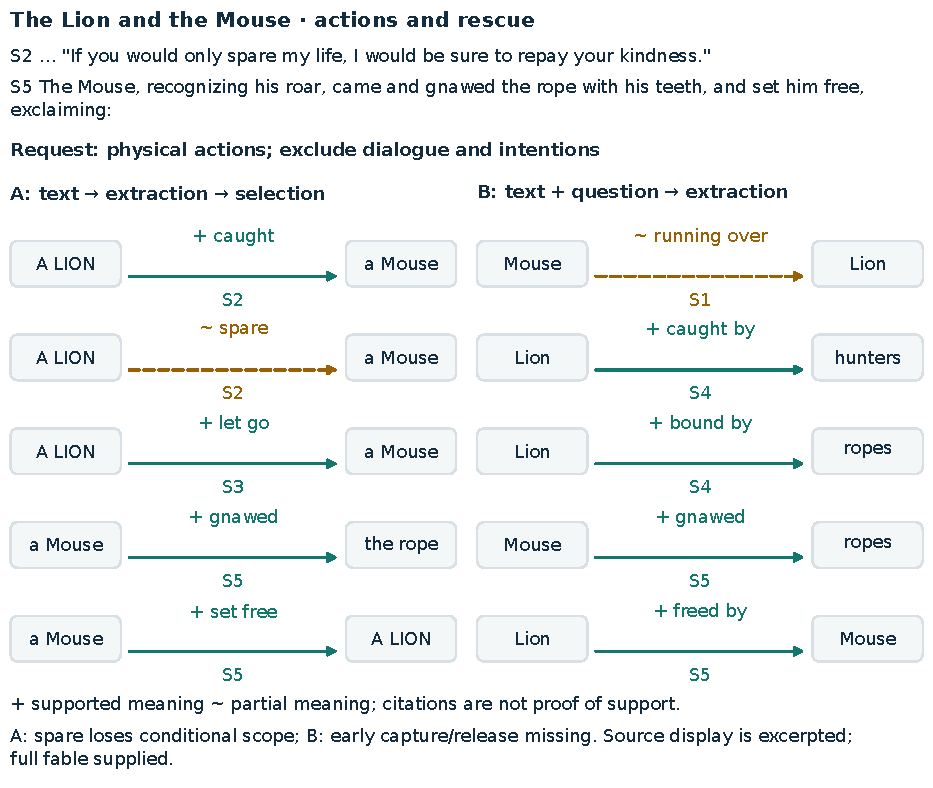
\includegraphics[width=\textwidth]{figures/fable.pdf}
\caption{Fable actions from pre-extract/select (A) and independent contextual extraction (B). + indicates supported meaning and $\sim$ partial meaning. Display: five of eight A records and all five B records. A's awakening, hunter capture and rope binding are omitted only from display. All predictions remain scored. Executed question: \FableQuestion\ Source display excerpts S2 and S5 from the complete supplied fable. The spare edge loses conditional scope and retains the misspelled key \texttt{valid until}. B loses the face-specific running endpoint and omits the early capture/release. Other displayed qualifications are null. Assessments are Codex-authored.}
\label{fig:fable}
\end{figure*}}
\newcommand{\HarborFigure}{
\begin{figure*}[!t]
\centering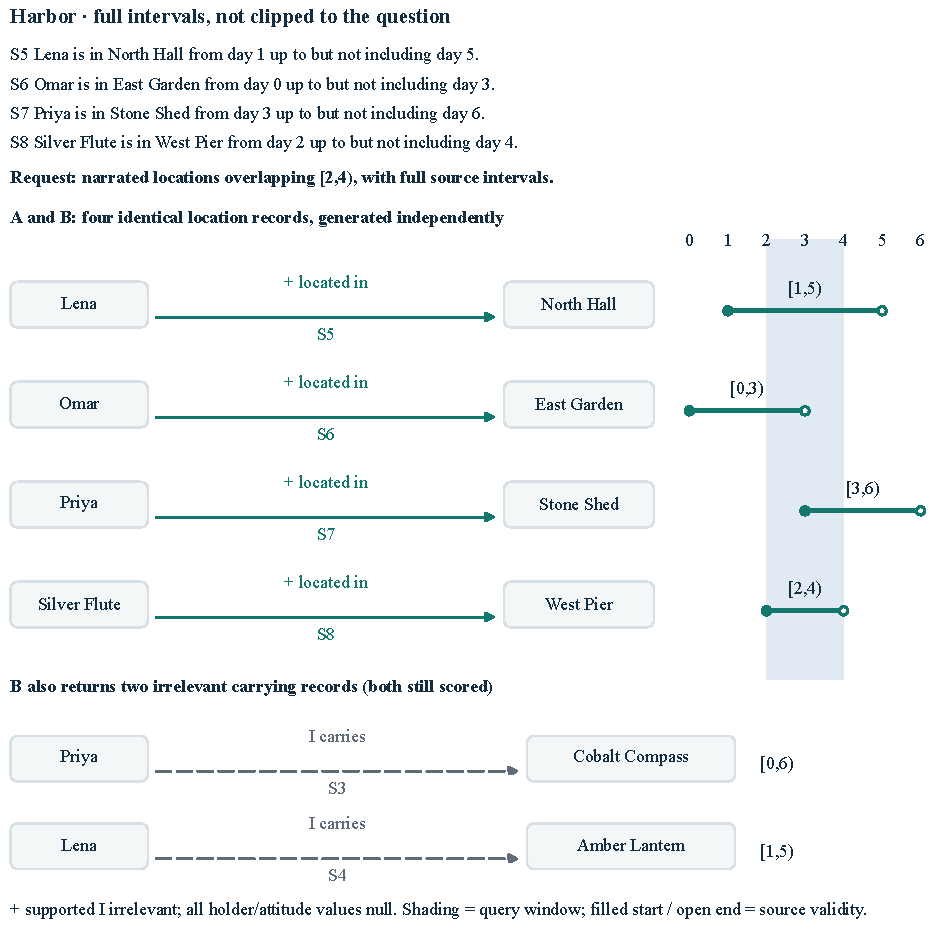
\includegraphics[width=\textwidth]{figures/harbor.pdf}
\caption{Harbor locations from pre-extract/select (A) and contextual extraction (B). Four independently generated records coincide and are shown in aligned rows. B also returns the two carrying edges below. Filled/open circles mark included/excluded bounds. Shading shows the query window, not rewritten validity. Executed question: \HarborQuestion\ Source display S5--S8 from the fourteen sentences supplied to both approaches. All six B predictions remain scored. + indicates supported meaning and I supported but irrelevant content. Holder and attitude are null throughout.}
\label{fig:harbor}
\end{figure*}}
\newcommand{\AliceFigure}{
\begin{figure*}[!t]
\centering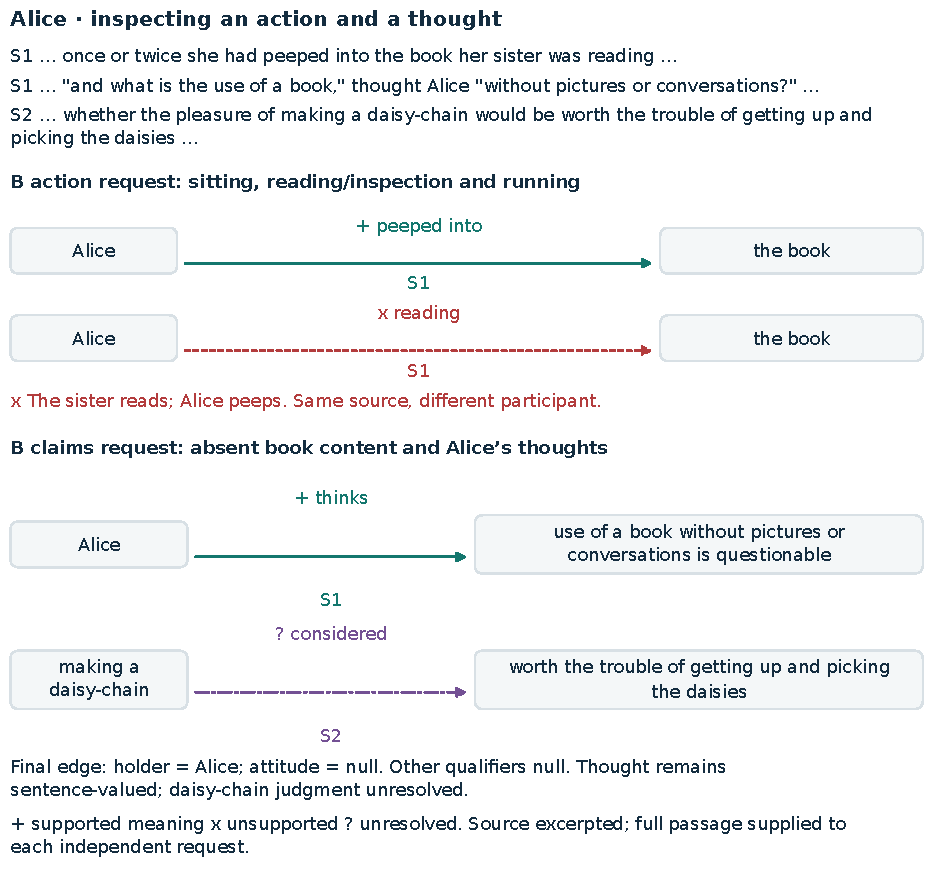
\includegraphics[width=\textwidth]{figures/alice.pdf}
\caption{Alice: independent contextual extraction (B) for two requests over identical complete evidence. Display: two of five action edges (two sitting edges and Rabbit running omitted) and two of three claims (book content omitted). All remain scored. Executed action question: \AliceActionQuestion\ Executed claims question: \AliceClaimQuestion\ Source excerpts are marked. + indicates supported meaning, x an unsupported participant, and ? unresolved consideration. The thought remains the actual sentence-valued object. All bounds are null. The final record has holder Alice and null attitude.}
\label{fig:alice}
\end{figure*}}

\newcommand{\aidraft}{\emph{AI-assisted preparation:} OpenAI Codex \cite{openai2025}; see Section~\ref{sec:disclosure}.}
\begin{document}
\title{Inspectable Narrative Graphs: Evidence-Linked Extraction and Contextual Selection}
\author{}
\keywords{Natural Language Processing, Knowledge Representation and Reasoning, Large Language Models, Visualization.}
\abstract{We present a narrative extraction workflow connecting readers' questions, generated relationships, temporal and attribution details, and visual inspection of evidence and errors. We compare extraction before seeing a question followed by fixed selection with independent contextual extraction on three synthetic stories and three short published passages. Assessment separates strict agreement with reference answers from preserved meaning, relevance and unresolved interpretation. All \CompactCalls\ story responses were parseable. Fixed selection matched every possession and dated location target without extras, whereas contextual answers retained irrelevant facts. On fable actions, strict F1 was \FableAFone\ for selection and \FableBFone\ for contextual extraction. Alice's contextual claims preserved \AliceBCoverage\ semantic targets despite zero strict F1. Prose parsing succeeded in \ProseParsed\ of \ProseCalls\ calls. The workflow makes these mixed results inspectable, including useful thought representations, incorrect participants and lost conditional scope. These small development comparisons identify concrete extraction and selection problems for further research. Reference annotations, assessments and manuscript preparation used OpenAI Codex \cite{openai2025}.}

\onecolumn\maketitle\normalsize\setcounter{footnote}{0}\vfill

\section{\uppercase{Introduction}}
\noindent A reader may want an account of who carries an object, a map of locations during an interval, or a summary of what a character believes. These are different information needs over the same narrative. A directed graph makes candidate relationships explicit, but a plausible arrow can conceal a mistake. Looking into a book is not equivalent to reading it; a character's belief about an object does not establish its location. The practical task is to extract a bounded, question-relevant view whose claims can be checked against the supplied text.

We present an implemented prototype that combines compact, evidence-linked extraction with selection and visual inspection. It compares two procedures: generating a query-blind fact collection and selecting its existing records (A), and independently generating from the same text plus a question (B). Readable endpoints, citations, temporal bounds and attribution make records inspectable. Coordinated views expose source wording, executed requests, actual graphs and assessment, including imperfect outputs. The contribution is not just drawing triples: it is the integration of question handling, qualification and source-linked error inspection, with separate measures of agreement and preserved meaning.

Our position is that useful narrative-graph prototypes should report both what their records preserve and what those records misrepresent, rather than making a single all-or-nothing verdict the condition for inspection. We investigate whether relevant relationships survive increasingly natural prose, whether contextual extraction improves selection, and what the graph reveals beyond strict matching. Results from short synthetic stories and published passages show useful extraction with mixed comparisons, incomplete attribution and substantive participant errors.

This is empirical work in progress on extraction and selection, not a demonstration of query-dependent ontology construction, general reliability or human usability. Richer ontology formation motivates subsequent research; a registered large benchmark and full-novel analysis have not been executed as part of this contribution. \aidraft

\FableFigure
\section{\uppercase{Related Work}}
\noindent Open information extraction introduced relational tuple extraction without a separately trained extractor for every target relation \cite{banko2007}. Language-model systems such as SPIRES use prompting and normalization to populate structured knowledge bases \cite{caufield2024}. Our prototype uses a smaller common record format and compares where the question enters the extraction process. It does not claim a new extraction model. Its distinctive emphasis is the inspectable connection between the question, extracted qualifications and several kinds of error.

Temporal and perspectival representation explain why bare tuples are insufficient. OWL-Time distinguishes instants, intervals and temporal ordering \cite{time2017}; GRaSP relates content to sources and perspectives \cite{fokkens2017}. These ideas motivate retaining source-supported validity and separating a narrated relationship from an attributed proposition. Our compact format covers explicit bounds and simple attribution, not the full expressive range of either framework.

Selection, filtering and coordinated views are established visual-analysis operations \cite{heer2012}. Here, edge selection connects a claim to its cited text while assessment remains a separate visual variable. A valid citation can still point to a sentence that fails to support the claim. This distinction makes both representation differences and incorrect participants visible. \aidraft

\section{\uppercase{Representation and Methods}}
\subsection{Evidence and Qualified Records}
\noindent Each request receives a complete selected story or contiguous excerpt, with numbered evidence spans. Literary wording is preserved. An output contains a list of facts with eight fields: \texttt{subject}, \texttt{relation}, \texttt{object}, \texttt{evidence\_ids}, \texttt{valid\_from}, \texttt{valid\_until}, \texttt{holder} and \texttt{attitude}. The model authors all these values; the runtime does not supply missing semantics from references.

For example, the following formatting illustration is authored, not a model result:
\begin{small}\begin{verbatim}
{"subject":"Nara", "relation":"carries",
 "object":"map", "evidence_ids":["X1"],
 "valid_from":2, "valid_until":5,
 "holder":null, "attitude":null}
\end{verbatim}\end{small}
Given explicit evidence, this expresses carrying over $[2,5)$, with start included and end excluded. A question window such as $[3,4)$ selects an overlapping record without clipping its source bounds. Intrinsic validity concerns when a relationship holds; event occurrence or observation alone does not establish its onset or duration. Unsupported bounds remain null, which means unspecified here, not timeless or false. Relative phrases such as ``shortly after'' are not converted to numerical validity, so their temporal information may be lost by this format.

For belief, the subject--relation--object expresses the believed relationship; holder names the believer and attitude is \texttt{believes}. Direct narration uses null holder and attitude without implying that characters know, or do not know, the fact. A narrated mental or speech act may instead be an explicit relationship, but its uncertain content must not become established reality. The prompt asks for pronoun resolution only when the excerpt makes the referent clear. Missing nullable fields are interpreted as unspecified by the frozen qualification matcher, while required-field compliance separately records their absence. No known bound or holder is filled from a reference.

\subsection{Two Question-Handling Procedures}
\noindent A first extracts all explicitly supported relationships without seeing the questions. Its actual output is frozen before any contextual request is sent. CPU selection then retains existing records by relation category, requested entity, attribution status or explicit interval overlap. Synthetic rules distinguish possession, dated location and belief/narration; prose rules use passage-appropriate lexical action and claim categories. These fixed rules do not infer relationships, repair meanings or consult reference answers.

B independently receives the same complete evidence and one question, and is instructed to return only the relationships needed to answer it. It never consumes A's graph. Both procedures use the same representation, model and general authoring conventions. Prompts, questions, selectors and call order are frozen before each batch. All query-blind calls precede contextual transmission. Each request is executed once without adaptive repair; a failed A output does not block B.

The experiments use \texttt{Qwen/Qwen3-8B-AWQ} in nonthinking mode \cite{qwen2025,qwenmodel}, served by vLLM \cite{kwon2023} on one RTX 4090. Temperature is \Temperature, top-p \TopP, top-k \TopK, and seed \Seed. Each request reserves \OutputTokens\ output tokens within a \ContextTokens-token context. The pinned model revision is recorded in the appendix. Ordinary JSON is requested without a guided schema. The same short, unrelated formatting example is supplied to A and B; it contains no tested reference answer.

\subsection{Inspecting Actual Output}
\noindent Graph edges retain generated direction, names, citations and qualifications. Only identical endpoint strings share a display identity; aliases are not inferred to tidy the picture. Sentence-valued objects remain literal nodes. Colours together with symbols and line styles distinguish supported, partial, unsupported, unresolved and supported-but-irrelevant content. A citation highlight is a navigation aid, not verification. Errors and missing targets appear alongside the graph, not as corrected model edges. Labelled display subsets do not change scoring denominators. The figures below use faceted edges to keep long names readable at conference size. \aidraft

\HarborFigure
\section{\uppercase{Evaluation}}
\subsection{Materials and Annotation}
\noindent The compact-story v2 comparison uses Harbor, Orchard and Museum, each with \StorySentences\ short evidence sentences. Three questions per story request possession, interval-dependent location, and belief contrasted with narration. Harbor and Orchard had been used in development; Museum adds different sentence ordering and bindings frozen before this batch. Earlier simple ladders supplied development context but are not pooled with these results or with historical syntax-recovered outputs.

The published-prose comparison uses the complete Lion and Mouse fable in Townsend's translation (\FableWords\ words), the opening of \emph{Alice's Adventures in Wonderland} (\AliceWords\ words), and a contiguous opening passage from The Red-Headed League in \emph{The Adventures of Sherlock Holmes} (\HolmesWords\ words) \cite{aesop,carroll,doyle}. These passages were selected before execution for understandable participants, actions and thought or dialogue. Two questions per passage address bounded action and claim information. This is extraction from published fiction, not verification of real events.

Evidence, question scope, reference alternatives and normalization were frozen before generation. References and subsequent response-linked semantic assessments were Codex-authored \cite{openai2025}, not independently human-validated. Synthetic source inventories distinguish supported but irrelevant records from unsupported ones. Prose reference coverage is question-scoped; unmatched wording alone is not treated as false. Ambiguous judgments, including Holmes's vocative and Alice's daisy-chain consideration, remain open to author review.

\subsection{Agreement, Meaning and Failure}
\noindent Strict qualified-fact scoring matches predictions one-to-one to frozen alternatives. It requires the normalized relationship, evidence set and temporal/attribution values to agree. Precision is matches divided by all predictions; recall is matches divided by reference targets; F1 is their harmonic mean. Incorrect, duplicate, irrelevant and unresolved predictions remain in the denominator. Omissions reduce recall. Bare-relationship measures ignore qualifications and citations. Strict F1 therefore measures agreement with this annotation contract, not the proportion of statements that are factually true.

Semantic assessment separately records supported, partially supported, unsupported and unresolved content, qualification errors and relevance. Target coverage counts distinct target meanings explicitly preserved; one combined object may cover several targets while still being one prediction. Partial support is not full target coverage. Absence of a known contradiction is not evidence of support. These measures expose useful content without inventing missing semantics or making matcher equivalence more permissive after seeing which procedure benefits.

Strict parsing rejects malformed JSON, duplicate keys and non-JSON constants. A narrowly permitted derived recovery can remove a trailing comma immediately before a closing delimiter outside strings, retaining raw bytes and an edit record. It cannot complete truncated content or remove extra braces. Neither main batch required such recovery. Unparseable results have unavailable graph scores, not the semantics of an intentionally empty graph.

The analysis is descriptive. These are purposively selected development examples, not independent repeated trials of a population effect. Questions sharing a story and outputs reused by selection are dependent. We do not use significance tests or treat individual records as independent experimental units. \aidraft

\AliceFigure
\section{\uppercase{Results}}
\subsection{Synthetic Selection and Qualifications}
\noindent All \CompactCalls\ compact-story outputs are strictly parseable. A matches every possession and dated-location target without extras (Table~\ref{tab:compact}). B commonly retrieves the requested physical relationships but returns irrelevant facts in every contextual answer. Orchard's location answer also omits a target: recall is \OrchardLocationRecall. The fresh Museum story shows the same over-selection limitation as the earlier stories.

\begin{table*}[t]
% Positive inset keeps the top caption within the nominal text margin.
\vspace*{6pt}
\caption{Compact-story v2 strict qualified-fact scores. A: pre-extract/select. B: contextual extraction. $n$ includes every prediction. Targets per story: possession 5, location 4, belief/reality 4. No historical recoveries are pooled.}\label{tab:compact}
\centering\small
\begin{tabular}{llrrrrrrrr}\toprule
Story & Question & $n_A$ & $P_A$ & $R_A$ & $F1_A$ & $n_B$ & $P_B$ & $R_B$ & $F1_B$\\\midrule
Harbor & Possession & 5 & 1.000 & 1.000 & 1.000 & 10 & 0.500 & 1.000 & 0.667 \\
Harbor & Location & 4 & 1.000 & 1.000 & 1.000 & 6 & 0.667 & 1.000 & 0.800 \\
Harbor & Belief/reality & 5 & 0.000 & 0.000 & 0.000 & 14 & 0.143 & 0.500 & 0.222 \\
Orchard & Possession & 5 & 1.000 & 1.000 & 1.000 & 12 & 0.417 & 1.000 & 0.588 \\
Orchard & Location & 4 & 1.000 & 1.000 & 1.000 & 5 & 0.600 & 0.750 & 0.667 \\
Orchard & Belief/reality & 4 & 1.000 & 1.000 & 1.000 & 13 & 0.154 & 0.500 & 0.235 \\
Museum & Possession & 5 & 1.000 & 1.000 & 1.000 & 13 & 0.385 & 1.000 & 0.556 \\
Museum & Location & 4 & 1.000 & 1.000 & 1.000 & 5 & 0.800 & 1.000 & 0.889 \\
Museum & Belief/reality & 4 & 0.000 & 0.000 & 0.000 & 14 & 0.143 & 0.500 & 0.222 \\\bottomrule\end{tabular}\end{table*}


Among emitted records with identifiable explicitly timed sources, \IntervalsKept\ of \IntervalsEligible\ preserve their full intervals, including irrelevant records. This is conditional preservation, not temporal recall over every reference. Figure~\ref{fig:harbor} shows how an intact interval can coexist with a relevance error. Attribution is less stable: Orchard's pre-extraction decomposes beliefs correctly, whereas Harbor and Museum use sentence-valued belief objects that disrupt selection. This explains why the physical-fact result does not extend to every belief view.

\subsection{Published Prose and Partial Meaning}
\noindent Of \ProseCalls\ prose responses, \ProseParsed\ are strictly parseable. Holmes's pre-extraction and contextual action answer end with an extra closing brace. Their unavailable views remain in Table~\ref{tab:prose}; failure of the shared pre-extraction affects both A questions. The parseable Holmes claims answer has partial and unresolved content rather than fully covered targets.

\begin{table*}[t]
\caption{Published prose: strict qualified-fact precision, recall and F1, separate from Codex-authored semantic support (S), partial support (P), unsupported (X), unresolved (U), and semantic target coverage. NA = unavailable due to parse failure, not an empty graph. All parseable predictions have valid evidence IDs; that does not establish support.}\label{tab:prose}
\centering\small\begin{tabular}{lllrrrrrr}\toprule
Passage & Question & Method & $n$ & Precision & Recall & F1 & S/P/X/U & Coverage\\\midrule
Alice & Actions & A & 2 & 0.500 & 0.200 & 0.286 & 2/0/0/0 & 3/5 \\
Alice & Actions & B & 5 & 0.400 & 0.400 & 0.400 & 3/1/1/0 & 3/5 \\
Alice & Claims & A & 4 & 0.000 & 0.000 & 0.000 & 2/2/0/0 & 1/4 \\
Alice & Claims & B & 3 & 0.000 & 0.000 & 0.000 & 2/0/0/1 & 3/4 \\
Fable & Actions & A & 8 & 0.625 & 0.625 & 0.625 & 6/1/0/1 & 6/8 \\
Fable & Actions & B & 5 & 0.400 & 0.250 & 0.308 & 4/1/0/0 & 4/8 \\
Fable & Claims & A & 1 & 0.000 & 0.000 & 0.000 & 1/0/0/0 & 2/5 \\
Fable & Claims & B & 4 & 0.000 & 0.000 & 0.000 & 1/3/0/0 & 0/5 \\
Holmes & Actions & A & NA & NA & NA & NA & NA & NA \\
Holmes & Actions & B & NA & NA & NA & NA & NA & NA \\
Holmes & Claims & A & NA & NA & NA & NA & NA & NA \\
Holmes & Claims & B & 3 & 0.000 & 0.000 & 0.000 & 0/1/0/2 & 0/5 \\\bottomrule\end{tabular}\end{table*}


For fable actions, A has strict F1 \FableAFone\ versus \FableBFone\ for B, and semantic coverage \FableACoverage\ versus \FableBCoverage. Both capture the later rescue, but B omits the early capture and release. A's unqualified \texttt{spare} relation loses the scope of the Mouse's conditional plea (Figure~\ref{fig:fable}). Some supported passive formulations also fail strict matching: semantic preservation and reference agreement are not interchangeable.

Alice shows a different comparison. B's claims preserve \AliceBCoverage\ semantic targets, compared with \AliceACoverage\ for A, despite zero strict F1 for both. The thought object preserves rhetorical meaning but not the requested decomposition. B also assigns reading to Alice instead of her sister, and the daisy-chain record leaves open whether considering worth has become judging it worthwhile (Figure~\ref{fig:alice}). More covered meaning can therefore accompany a substantive error or unresolved interpretation.

\subsection{Cost of the Presented Experiments}
\noindent The two main batches comprise \MainCalls\ generations and \MainAllocation\ allocated GPU seconds. Compact stories used \CompactAllocation\ seconds and prose \ProseAllocation\ seconds; summed request times were \CompactRequest\ and \ProseRequest\ seconds respectively. Allocation includes loading, checks, service idle time and shutdown. Pre-extractions reused across questions are counted once. These costs exclude earlier ladders and whole-project development history, and do not establish full-study feasibility or production-tail latency. \aidraft

\section{\uppercase{Discussion and Limitations}}
\noindent The implemented workflow makes extraction quality inspectable along several axes. A relationship can be semantically useful yet fail a strict match; an attractive graph can assign an action to the wrong participant. Reporting both is more informative than requiring a perfect graph before showing anything or treating every unmatched wording as false. For the intended reader task, the evidence link enables examination of these differences, although a user study would be needed to demonstrate improved comprehension.

The comparison also exposes limitations of fixed selection. It cannot recover an omitted fact or repair an attribution error. In the fable claims view, its exact subject filter expects ``Lion'' and rejects ``A LION'', discarding useful records. In Alice, feeling records embedding actions can be excluded by the action filter. Thus the results concern these particular implementations, including selector brittleness, rather than an inherent advantage of pre-extraction. Conversely, B's repeated over-selection shows that a prominent question and compact format alone do not guarantee relevance.

The small, purposive samples limit inference. Several examples were reused during development, familiar prose may have been in model training, and there is one generation per request. Shared AI assistance in implementation, annotation and assessment creates possible correlated blind spots. Reference scope and semantic interpretations still require author and independent review. The compact fields cannot faithfully encode every relative time phrase, nested perspective or event structure. Our display does not fix those representational limits, and no participant evaluation demonstrates usability.

Next work should independently review reference coverage, freeze fresh passages and compare targeted improvements in participant, attribution and relevance handling without passage-specific answer hints. Query-dependent formation of entities, events and schemas requires a different comparison; differences between these extracted views alone do not establish it. \aidraft

\section{\uppercase{Conclusion}}
\noindent We demonstrate compact evidence-linked narrative extraction, fixed selection versus independent contextual extraction, and visual inspection of qualifications and errors. Synthetic intervals survive in the observed timed records, while published prose provides useful action and thought information alongside omissions, wrong participants and syntax failures. The simpler selector performs better on several questions; contextual extraction preserves additional meaning in Alice's claims. These mixed results support an inspectable work-in-progress prototype and the joint reporting of strict agreement, preserved meaning, relevance and uncertainty, not contextual superiority or general reliability. \aidraft

\section{\uppercase{AI Use and Annotation Provenance}}
\label{sec:disclosure}
\noindent OpenAI Codex \cite{openai2025} assisted implementation, analysis and figure-generation code, reference annotation, semantic assessment, and drafting and editing all manuscript sections including the abstract and captions. This was substantive assistance, not spelling correction. The figures are deterministic renderings of retained records, not newly generated model illustrations. Qwen generated the experimental fact collections. Codex-authored judgments are explicitly distinguished from human validation; pending semantic decisions have not been marked reviewed. Responsibility for the submitted work remains with its human author(s). No identifying acknowledgments are included in this review version.

\bibliographystyle{apalike}
{\small\bibliography{references}}
\section*{APPENDIX}
\noindent Reproducibility identifier: Qwen3-8B-AWQ snapshot \texttt{4da05a8edb55c6046cce9585}\allowbreak\texttt{86c33b61da07bb79}; vLLM 0.10.2 and Transformers 4.55.2. Requests use the pinned chat template with \texttt{enable\_thinking=False}. Complete model messages, output records, frozen alternatives and assessments are retained in a separately prepared anonymous companion. Its eligibility as an additional upload has not been established; all principal methods, results and limitations are included here. Preparation used Codex \cite{openai2025}.
\end{document}
